\documentclass[letterpaper,twocolumn,10pt]{article}
\usepackage{usenix,epsfig,endnotes}
\usepackage{graphicx}
\usepackage[labelfont=bf]{caption}

\setlength\parindent{0pt}

\begin{document}

%don't want date printed
\date{}

%make title bold and 14 pt font (Latex default is non-bold, 16 pt)
\title{\Large \bf ECE 225A Project Report - California Housing Prices}

\author{
{\rm Kirtan Shah}\\
Department of Electrical and Computer Engineering, University of California, San Diego
}

\maketitle

% Use the following at camera-ready time to suppress page numbers.
% Comment it out when you first submit the paper for review.
\thispagestyle{empty}


\subsection*{Abstract}

\section{Introduction}
The California housing market has long been a subject of interest for economists, policymakers, and residents alike. 
Its complexity, driven by factors ranging from economic conditions to geographical desirability, presents a rich field for data analysis. 
This paper presents an exploratory data analysis of the California Housing Prices dataset, a comprehensive collection of housing-related statistics from the 1990 California census. 
For this project, I focus on uncovering insights into patterns within the data, especially in relation to median house values across different census areas in California. 
Through data preprocessing, statistical modeling, and visualization techniques, I explore key factors such as room count, population, median income, and geographical location. 
I also develop and present a predictive model for median house values based such factors, which provides further insight into the complex dynamics of California's housing market.



\section{Dataset}
The dataset, provided by the US Census and available on Kaggle, comprises housing-related statistics for different blocks in California.
Each entry represents statistics for a group of homes in a given block.

\subsection{Dataset Description}
These variables include the following:
\begin{itemize}
    \item Latitude and longitude
    \item Median house age within block
    \item Total rooms, total bedrooms
    \item Total population
    \item Number of households in block
    \item Median income for households in block
    \item Median house value for households in block
    \item Ocean proximity (<1H OCEAN, INLAND, ISLAND, NEAR BAY, NEAR OCEAN)
\end{itemize}

% figure for image
\begin{figure}[h]
\centering
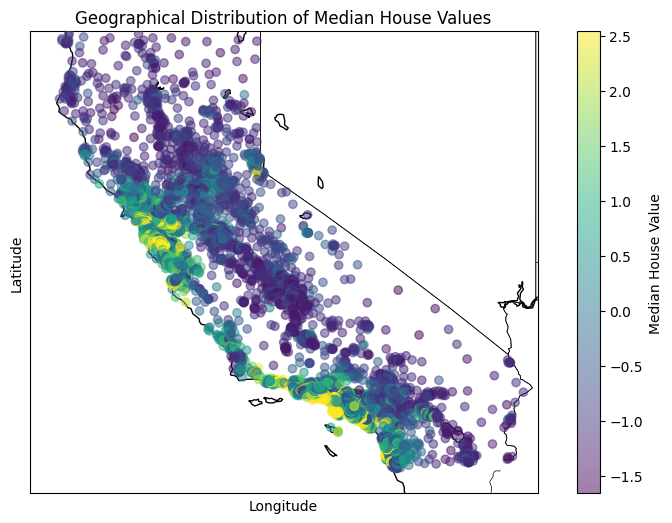
\includegraphics[width=0.5\textwidth]{images/california_map.png}
\caption{Visualization of California median house values}
\label{fig:california_map}
\end{figure}

The dataset contains 20640 entries corresponding to a different census block, each with the features described above.

\subsection{Exploratory Data Analysis}

Here it comes~\cite{Einstein}.  


\section{Code}
The code for this project is attached in the form of a Jupyter notebook in the Appendix.


{\footnotesize \bibliographystyle{acm}
\bibliography{sample}}

\appendix
\section*{Appendix}

\end{document}







